\documentclass[12pt,fleqn]{article}\usepackage{../../common}
\begin{document}
Materyel Mekaniği - 4

Yapıların stres, kaykılma fiziğini kullanarak Euler-Bernoulli kirişlerinden
bahsedildi, ve bir diferansiyel denklem elde edildi. Bu denklem kesin (exact)
olarak çözülebilir fakat bazı durumlarda bu denklem çözümü zor olabilir. Kesin
metotlar yerine yaklaşık metotlara bakmak faydalı olacaktır.

Rayleigh-Ritz metotu diferansiyel denklemleri yaklaşıksal olarak çözmenin
yöntemlerinden biridir. Metot bunu sistemin potansiyel enerjisi $\Pi$'yi
minimize ederek yapar [1, Ders 3]. Potansiyel enerji sistemin toplam iç gerilme
enerjisi eksi sistem üzerinden yapılan iş olarak hesaplanabilir,

$$
\Pi = \int_\Omega \bar{U} \ud x - W
$$

Bu noktada aklimiza pek cok soru gelebilir - niye potansiyel enerji minimize
ediyoruz, is gerilme enerjisi ve yapilan is nasil hesaplanir, potansiyel enerji
nasil minimize edilir gibi..

Potansiyel Enerji ve Denge

İlk önce denge bağlamında potansiyel enerjinin ne demek olduğunu işleyelim.

Potansiyel enerji $\Pi$ sistemin stabilitesi ile alakalıdır. Mesela alttaki
resim stabilite konusunu işleyen her ders kitabında vardır, bir kapta duran topu
aldım, yukarı doğru çıkatıp (bordo renk) aşağı bıraktım, top kabin dibine gidip
orada kalacaktır (kırmızı renk). 

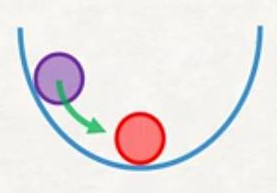
\includegraphics[width=10em]{phy_020_strs_04_01.jpg}

Yani top ilk denge konumuna dönecektir, ve o durumda potansiyel enerjisi minimum
olmuştur deriz ve bu denge stabil bir dengedir. 


[devam edecek]

Kaynaklar

[1] Petitt, {\em Intro to the Finite Element Method}, University of Alberta,
    \url{https://www.youtube.com/watch?v=2iUnfPRk6Ro&list=PLLSzlda_AXa3yQEJAb5JcmsVDy9i9K_fi}

\end{document}
